\documentclass{article}
\usepackage{graphicx}

\title{Clase Práctica 2}
\author{Javier Alejandro Oramas López}
\date{}

\begin{document}
    \maketitle
    \section{}
    \[ \frac{\partial{T}}{\partial{t}} = -k(T-A) \]
    \[ \frac{\partial{T}}{T-A} = -k \partial{t} \]
    \[ \int \frac{\partial{T}}{T-A} = -\int k \partial{t} \]
    \[ \log{|T-A|} = -(kt+C) \]
    \[ T-A = e^{-kt+C} \]
    \[ T-A = \frac{e^-kt}{C} \]
    \[ T = \frac{1}{C}e^{kt} - A\]
    
\section{}
    \begin{enumerate}
        \item P: Población (cte)
        \item N: Personas Infectadas 
        \item P-N: Personas sanas
        \item k: cte de proporcionalidad
    \end{enumerate}

    \[ \frac{\partial{N}}{\partial{t}} = k(P-N)N \]
    \[ \int \frac{\partial{N}}{N(P-N)} = \int k(\partial{t}) \]
    \[ - \frac{1}{P} \left( - \ln{\frac{|N|}{|P|} + \ln{|\frac{N}{P} -1|}} \right) = kt +C\]
    \[ - \left( - \ln{\frac{|N|}{|P|} + \ln{|\frac{N}{P} -1|}} \right) = P(kt +C)\]
    \[ \ln{\frac{|N|}{|P|} - \ln{|\frac{N}{P} -1|}} = P(kt +C) \]
    \[ \ln(\frac{\frac{N}{P}}{\frac{N}{P} -1}) = P(kt +C)\]
    \[ \frac{\frac{N}{P}}{\frac{N}{P} -1} = e^{P(kt +C)}\]
    \[ \frac{N}{N-P} = e^{P(kt +C)}\]
    
\section{}

    \[ \frac{\partial{y}}{\partial{x}} = \sin{x-y} \]
    \[ \partial{y} = \sin{x-y}\partial{x} \]
    \[ \partial{y} - \sin{x-y}\partial{x} = 0\]
    \[ \partial{y} - \sin{x-y}\partial{x} = 0\]
    
    $t = x-y$

    $\partial{t} = \partial{x}-\partial{y}$

    $\partial{y} = \partial{x} - \partial{t}$

    \[ \partial{x} - \partial{t} - \sin{t}\partial{x} = 0\]
    \[  - \partial{t} - (1 - \sin{t})\partial{x} = 0\]
    \[  \partial{x} = \frac{\partial{t}}{1 - \sin{t}}\]
    \[  \partial{x} - \frac{\partial{t}}{1 - \sin{t}} = 0\]
    \[ \int \partial{x} - \int{\frac{\partial{t}}{1 - \sin{t}}} = 0 \]
    \[ x - \int{\frac{\partial{t}}{1 - \sin{t}}\frac{{1 + \sin{t}}}{1 - \sin{t}}} = 0 \]
    \[ x - \int{\frac{1 + \sin{t}}{1-\sin^{2}{t}}\partial{t}} = 0 \]
    \[ x - \int{\frac{1 + \sin{t}}{\cos^{2}{t}}\partial{t}} = 0 \]
    \[ x - \int{\frac{1}{\cos^{2}{t}}\partial{t}}+\int{\frac{\sin{t}}{\cos^{2}{t}}\partial{t}} = 0 \]
    \[ x - \int{\sec^{2}{t}\partial{t}}+\int{\cos^{-2}{t}\partial{t}} = 0 \]

    $ u = \cos{t}$

    $ \partial{u} = -\sin{t}$ 
    
    \[ x - \tan{t} + \frac{-u^{2+1}}{-2+1} = 0\]
    \[ x - \tan{t} + \frac{-cos^{-1}{t}}{-1} = 0\]
    \[ x - \tan{(x-y)} - \sec{(x-y)} = 0\]

\section{}
    \subsection{}
    \[ y^{'} = x+y \]
    \[ y^{'} = k , k = cte\]
    \[ x + y = k\]
    \[ y = k - x\]

    \[y(0) = 0\]
    \[ 0 = 0 + k\]
    \[k = 0\]

    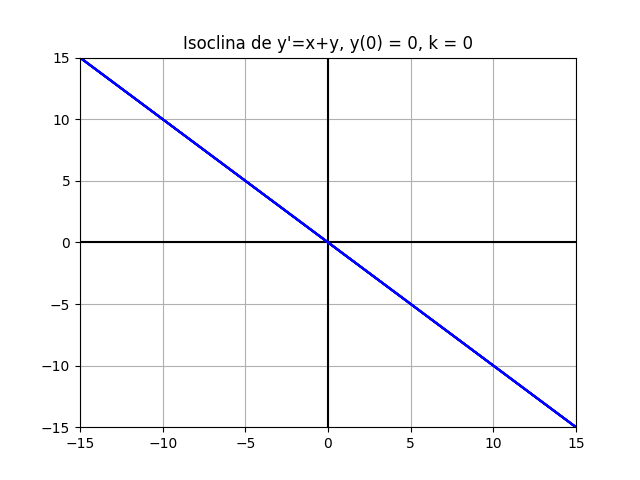
\includegraphics{isoclina_y'=x+y.png}

    \subsection{}
    \[y^{'} = 2x-y\]
    \[ y^{'} = k , k = cte\]
    \[ 2x - y = k\]
    \[ y = 2x - k\]

    \[y(4) = 0\]
    \[ 0 = 2(4) - k\]
    \[k = 8\]

    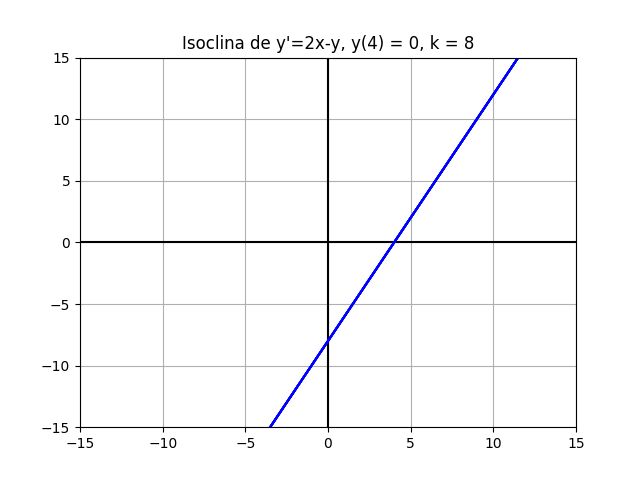
\includegraphics{isoclina_y'=2x-y.png}
    
\end{document}